\externaldocument{../appendix/chapter_app}
\startchapter{Modeling}
\label{chapter:Mod}
In this chapter, I modeled the communication of two running programs. The dual-trace captured from two interacting programs are also modeled in the perspective of communication analysis. The modeling are based on the investigation of some common used communication methods. The communication methods are divided into two categories based on their data transmission properties. This modeling are the foundation to decide how communications being identified from the dual-trace and how to present them to the user. The terminology of using in this chapter can be found in \ref{term}.

\section{Communication Categorization and Communication Methods}
The goal of this work is to identify the communications from the dual-trace. We need to understand the properties of the communications to identify them. In general, there are two types of communication: reliable and unreliable in the terms of their reliability of data transmission. The reason to divide the communication methods into these two categories is that the data transmission properties of the communications fall in different categories affect the mechanism of the data verification in the identification algorithm. In the following two subsections, I summarize the characteristics of these two communication categories. The communication methods list in Table\ref{methodsInCategories} will be discussed further to provide more concrete comprehension. 
\begin{table}[H]
\centering
\caption{Communication Methods Discussed in This Work}
\label{methodsInCategories}
\begin{tabular}{|l|l|}
 \hline
\textbf{Reliable Communication}& \textbf{Unreliable Communication}\\
 \hline
Named Pipes & Message Queue   \\
TCP &  UDP \\
 \hline
\end{tabular}
\end{table}


\subsection{Reliable Communication}\label{reliable}
A reliable communication guarantees the data being sent by one endpoint of the channel always received losslessly and in order to the other endpoint. For some communication methods, a channel can be closed without waiting the completion of all data transmission. With this property, the concatenated data in the receive stream of one endpoint should be the sub string of the concatenated data in the send stream of the other endpoint. Therefore, the send and receive data verification should be in send and receive stream level by comparing the concatenated received data of one endpoint to the concatenated sent data of another. 

\subsection{Unreliable Communication}\label{unreliable}
An unreliable communication does not guarantee the data being sent always arrive the receiver. Moreover, the data packets can arrive to the receiver in any order. However, the bright side of unreliable communication is that the packets being sent are always arrived as the origin packet, no data re-segmentation would happen. Accordingly, the send and receive data verification should be done by matching the data packets in a receive event to a send event on the other side.

\subsection{Communication Methods}
In this section, I describe the mechanism and the basic data transfer characteristics of each communication method in Table\ref{methodsInCategories} briefly. Moreover, data transfer scenarios are represented correspondingly in diagrams for each communication method. 
 
\subsubsection{Named Pipe}
A named pipe provides FIFO communication mechanism for inter-process communication. It can be one-way or duplex pipe which allows two programs send and receive message through the named pipe. \cite{khambattinamed}

The basic data transfer characteristics of Named Pipe are:
\begin{itemize}
  \item Bytes received in order
  \item Bytes sent as a whole trunk can be received in segments
  \item No data duplication
  \item Only the last trunk can be lost
\end{itemize}

Based on these characteristics, the data transfer scenarios of Named pipe can be summarized in Figure\ref{namedpipe}. 
\begin{figure}[H]
\centerline{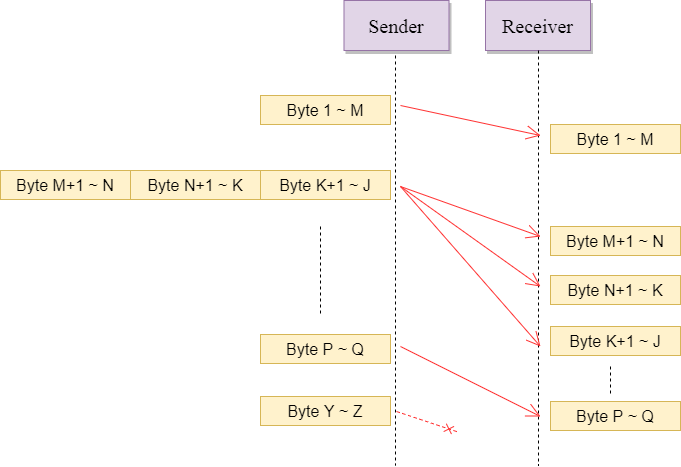
\includegraphics[scale=0.48]{Figures/namedpipe}}
\caption{Data Transfer Scenarios for Named Pipe}
\label{namedpipe}
\end{figure}

\subsubsection{Message Queue}
Message Queuing (MSMQ) is a communication method to allow applications which are running at different times across heterogeneous networks and systems that may be temporarily offline can still communicate with each other. Messages are sent to and read from queues by applications. Multiple sending applications can send messages to and multiple receiving applications can read messages from one queue.\cite{redkar2004pro} In this work, only one sending application versus one receiving application case is considered. Multiple senders to multiple receivers scenario can be divided into multiple sender and receiver situation. Both applications of a communication can send to and receive from the channel.

The basic data transfer characteristics of Message Queue are:
\begin{itemize}
  \item Bytes sent in packet and received in packet, no bytes re-segmented
  \item Packets can lost
  \item Packets received in order
  \item No data duplication
\end{itemize}
Based on these characteristics, the data transfer scenarios of Message Queue can be summarized in Figure\ref{msmq}.
\begin{figure}[H]
\centerline{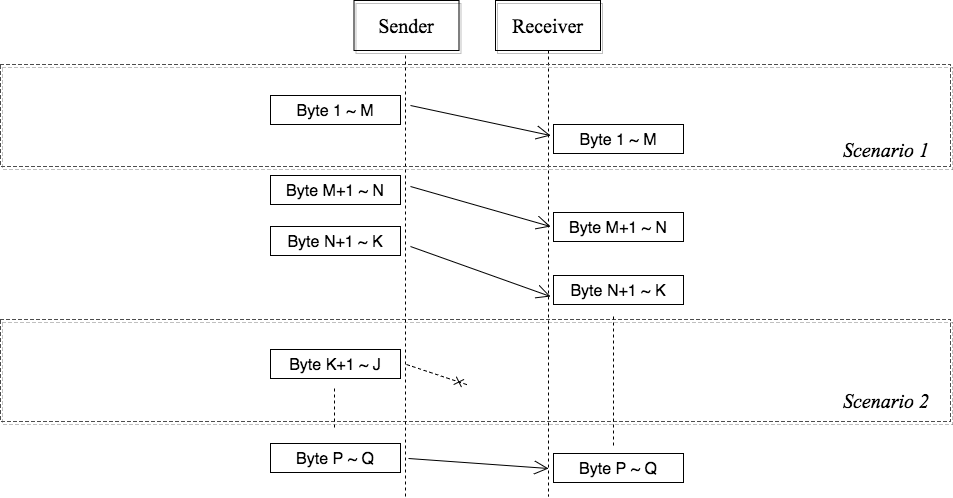
\includegraphics[scale=0.48]{Figures/msmq}}
\caption{Data Transfer Scenarios for Message Queue}
\label{msmq}
\end{figure}

\subsubsection{TCP}
TCP is the most fundamental reliable transport method in computer networking. TCP provides reliable, ordered, and error-checked delivery of a stream of octets between applications running on hosts in an IP network. The TCP header contains the sequence number of the sending octets and the acknowledge sequence this endpoint is expecting from the other endpoint(if ACK is set). The re-transmission mechanism is based on the ACK. 

The basic data transfer characteristics of TCP are:
\begin{itemize}
  \item Bytes received in order
  \item No data lost(lost data will be re-transmitted)
  \item No data duplication
  \item Sender window size is different from receiver's window size, so packets can be re-segmented
\end{itemize}

Based on these characteristics,  the data transfer scenarios of TCP can be summarized in Figure\ref{tcp}.
\begin{figure}[H]
\centerline{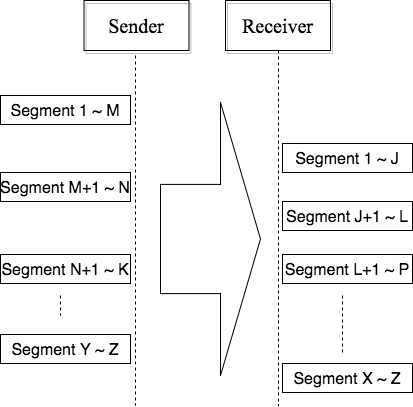
\includegraphics[scale=0.48]{Figures/tcp}}
 \caption{Data Transfer Scenarios for TCP}
\label{tcp}
\end{figure}

\subsubsection{UDP}
UDP is a widely used unreliable transmission method in computer networking. It is a simple protocol mechanism, which has no guarantee of delivery, ordering, or duplicate protection. This transmission method is suitable for many real time systems. 

The basic data transfer characteristics of UDP are:
\begin{itemize}
  \item Bytes sent in packet and received in packet, no re-segmentation
  \item Packets can lost
  \item Packets can be duplicated
  \item Packets can arrive receiver out of order
\end{itemize}

Based on these characteristics, the data transfer scenarios of UDP can be summarized in Figure\ref{upd}.
\begin{figure}[H]
\centerline{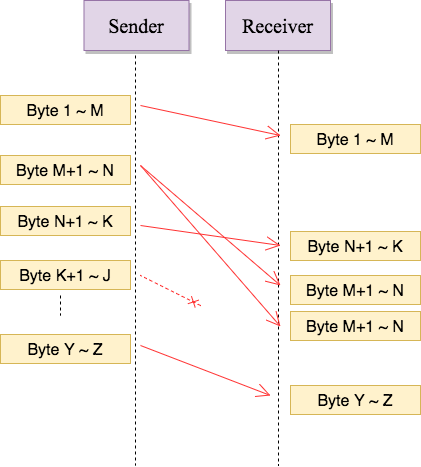
\includegraphics[scale=0.48]{Figures/udp}}
 \caption{Data Transfer Scenarios for UDP}
\label{upd}
\end{figure}

\section{Communication Model}\label{definition}
The communication of two programs is defined in this section. The communication in this work is data transfer activities between two running programs through a specific channel. Some collaborative activities between the programs such as remote procedure call is out of the scope of this research. Communication among multiple programs (more than two) is not discussed in this work. The channel can be reopened again to start new communications after being closed. However, the reopened channel will be treated as a new communication. The way that I define the communication is leading to the communication identification in the dual-trace. So the definition is not about how the communication works but what it looks like. There are many communication methods in the real world and they are compatible to this communication definition. 

\subsection{Communication Definition}
In the context of a dual\_trace, a communication is a sequence of data transmitted between two endpoints through a communication channel. The endpoints connect to each other using the identifier of this channel. We therefore defined a communication c as a tripled:

$c =<ch, e0, e1>$

where $e0$ and $e1$ are endpoints and where ch is the communication channel used (e.g. a named piped located at /tmp/pipe).

For the purpose of modelling the trace, the endpoints $e_0$ and $e_1$ are defined in terms of three properties: the handle created within a process for the endpoint for subsequent operations(such as data send and receive), the data stream received and the data stream sent. Therefore, we define an endpoint e as a triplet:

$ e =<handle, d_r, d_s>$

From the point of view of a trace, a data stream is a sequence of events that send or receive a package. Each package is composed contains data that is being sent or received (its payload). Hence, we can define a data stream $d$ as a sequence of $n$ packages:

$ d = (pk_1, pk_2, ..., pk_n)$ 

Note that this is the sequence of packages as seen from the end-point and might be different than the sequence of packages seen in the other end point, specially where there is package reordering or loss.

Each package has several attributes:
\begin{itemize}
\item \textit{Relative time(it was sent or received):} In a trace, we do not have absolute time for an event. However, we know when when an event (i.e. sending or receiving a package) has happened with respect to another event. we will use the notation 

$time(pkg)$ 

to denote this relative time. Hence, if 

$i < j $

, then 

$time(pk_i) < time(pk_j)$

\item \textit{Payload:} Each package has a payload (the data being sent). This payload can be modeled as a string contained in the package.we will use the notation 

$pl(pkg)$ 

to denote this payload. 

\end{itemize}


\subsection{Communication Properties}
The properties of the communications can be described based on the definition of the communication.

\subsubsection{Properties of reliable communication:}
A reliable communication guarantees that the data sent and received between a package happens without loss and in the same order.

For a given data stream, I will define the data in this stream as the concatenation of all the payloads of all the packages in this stream, in the same order, and denote is as $data(d)$.

Given $ d = <pk_1, pk_2, ..., pk_n>$, $data(d) = pl(pk_1) \cdot pl(pk_2)\cdot \ldots \cdot pl(pk_n)$


\begin{itemize}
 \item \textit{ Content Preservation:} for a communication:

$c = <ch, <h0, dr0, ds0>, <h1, dr1, ds1>>$

the received data should always be a prefix (potentially equal) of the data sent:

$data(dr0)$ is a prefix of $data(ds1)$  and

$data(dr1)$ is a prefix of $data(ds0)$

 \item \textit{Timing Preservation:} at any given point in time, the data received by an endpoint should be a prefix of the data that has been sent from the other:
 
for a sent data stream of size $m$, $ds= <pks_1, pks_2, ... pks_m>$ that is received in data stream of size $n$, $dr = <pkr_1, pkr_2, ... pkr_n>$

for any $k \in {1..n}$, there must exist $j \in {1..m}$ such that: $pks_j$ was sent before $pkr_k$ was received:

$  time(pks_j) < time(pkr_k)$

  and

$  data(<pkr_1, pkr_2, ..., pkr_k>)$ is a prefix of $data(<pks_1, pks_2, ..., pks_j>)$

  In other words,at any given time, the recipient can only receive at most the data has been sent.

\end{itemize}

\subsubsection{Properties of unreliable communication:}
In unreliable communication sender and receiver are not concerned with the concatenation of packages. Instead, they treat each package independent of each other.
\begin{itemize}
 \item \textit{ Content Preservation:} a package that is received should have been sent:

for a sent data stream of size $m$, $ds= <pks_1, pks_2, ... pks_m>$ that is received in data stream  of size $n$, $dr = <pkr_1, pkr_2, ... pkr_n>$

for any $pkr_j \in dr$ there must exist $pks_i \in ds$

We will say that the $pkr_j$ is the matched package of $pks_i$, and vice-versa, $pks_i$ is the matched package of $pkr_j$, hence

$match(pkr_j) = pks_i$  and

$match(pks_i) = pkr_j$

 \item \textit{Timing Preservation:}  at any given point in time, packages can only be received if they have been sent

  for a sent data stream of size $m$, $ds= <pks_1, pks_2, ... pks_m>$ that is received in data stream of size $n$, $dr = <pkr_1, pkr_2, ... pkr_n>$

  for any $k \in {1..n}$, $time(match(pkr_j)) < time(pkr_j)$

In other words, the match of the received package must has been sent before it is received.

\end{itemize}



In the following two examples, $h0$ and $h1$ are the handles of the two endpoints $e0$ and $e1$ of the communications. $ds0$, $dr0$ and $ds1$, $dr1$ data streams of the endpoints $e0$ and $e1$. The string payloads are the strings represented in blue and red in the figures. 

Figure\ref{reliableexample} is an example of the reliable communication. 

The payloads of the packages are:

$pl(pks0_1)=``ab"$, $ pl(pks0_2)=``cde"$, $pl(pks0_3)=``fgh"$;

$pl(pkr1_1)=``abc"$, $pl(pkr1_2)=``def"$, $pl(pkr1_3)=``gh"$ .

and 

$pl(pks1_1)=``mno"$, $pl(pks1_2)=``pqr"$, $pl(pks1_3)=``stu"$;

$pl(pkr0_1)=``mnop"$, $pl(pkr0_2)=``qrstu"$. 

on the other direction. Their properties:

$pl(pks0_1) \cdot pl(pks0_2) \cdot pl(pks0_3) = pl(pkr1_1) \cdot pl(pkr1_2) \cdot pl(pkr1_3) = ``abcdefgh"$ and 

$pl(pks1_1) \cdot pl(pks1_2) \cdot pl(pks1_3) = pl(pkr0_1) \cdot pl(pkr0_2) = ``mnopqrstu"$. 

satisfy the content preservation. 

The relative time relationship of the packages are: 

$time(pks0_1) < time(pks0_2) < time(pkr1_1)< time(pks0_3) < time(pkr1_2) < time(pkr1_3) $;

$time(pks1_1) < time(pks1_2) < time(pkr0_1)< time(pks1_3) < time(pkr0_2)$. 

The fact that
 
$pl(pkr0_1) = ``mnop"$ is the prefix of $pl(pks1_1) \cdot  pl(pks1_2) = ``mnopqr"$,

$pl(pkr0_1) \cdot pl(pkr0_2)=``mnopqrstu"$ is the prefix of(is this case identical to ) $pl(pks1_1) \cdot pl(pks1_2) \cdot pl(pks1_3) = ``mnopqrstu" $,  

$pl(pkr1_1)=``abc"$ is the prefix of $pl(pks0_1 \cdot pl(pks0_2) = "abcde"$,  

$pl(pkr1_1) \cdot pl(pkr1_2)= ``abcdef"$ and  $pl(pkr1_1) \cdot pl(pkr1_2) \cdot pl(pkr1_3) = ``abcdefgh"$ are  the prefix of  $pl(pks0_1) \cdot pl(pks0_2) \cdot pl(pks0_3)= ``abcdefgh"$

satisfy the timing preservation. 

\begin{figure}[H]
\centerline{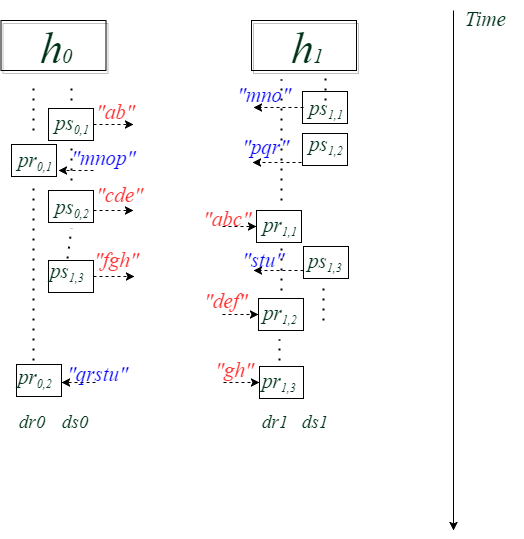
\includegraphics[scale=0.55]{Figures/reliableexample}}
\caption{Example of Reliable Communication}
\label{reliableexample}
\end{figure}

Figure\ref{unreliableexample} is an example of the unreliable communication. In this example:

$pkr1_1 = pks0_2=``cde"$, $time(pkr1_1) > time(pks0_2)$; 

$pkr1_2 = pks0_3=``fi"$, $time(pkr1_2) > time(pks0_3)$;

$pkr0_1 = pks1_1=``gh"$, $time(pkr0_1) > time(pks1_1)$;

$pkr0_2 = pks1_2=``ijklm"$, $time(pkr0_2) > time(pks1_2)$;

$pkr0_3 = pks1_3=``n"$, $time(pkr0_3) > time(pks1_3)$.

All of these satisfy the content preservation and timing preservation of the unreliable communication.
\begin{figure}[H]
\centerline{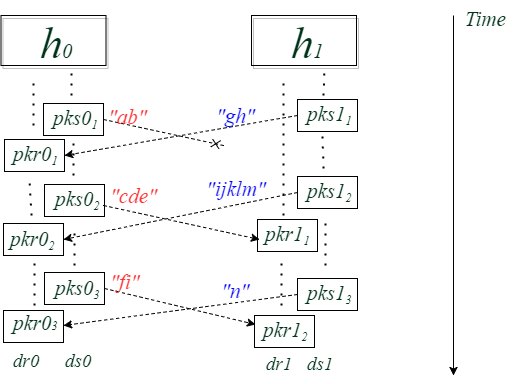
\includegraphics[scale=0.55]{Figures/unreliableexample}}
\caption{Example of Unreliable Communication}
\label{unreliableexample}
\end{figure}

\section{Dual-Trace Model}
In this section, I model the execution trace in the dual-trace. The modeling aims at identify the communications from the information summarized in the model. 

Before the modeling, I describe the facts of the dual-trace being analyzed. The traces in a dual-trace are in assembly level. One dual-trace contains two execution traces. There is no timing information of these two traces which means we don't know the time-stamps of the events of these two traces and can not match the events from both sides by time sequence. However the captured instructions in the trace are ordered in execution sequence. The execution traces contain all executed instructions as well as the corresponding changed memory by each instruction. Additionally, system calls are also captured by instruction id, which means if .dll or .exe files are provided, the system function calls can be identified with function names. Memory states can be reconstructed from the recorded memory changes to get the data information of the communication. 

In this model, a $dual\_trace$ consist of two execution traces which are $\left\lbrace trace_{x}: x= 0,1 \right\rbrace $ . An execution $trace$ is defined as a sequence $(line_{k}, 0 \leqslant k \leqslant K)$. $line_{k}$ in a $trace$ is a 3\_tuple $\langle ins, mem, inf \rangle$ where $ins$ is the assembly instruction, $mem$ is memory changed by this instruction and $inf$ is function call information. This information includes an indicator of function call and return and the function's name if applicable. A function $eventfilter \left( \right) $ is defined to generate the event level trace $event\_trace_{x}$ from the original $trace_{x}$. So that $event\_trace_{x} = eventfilter\left( trace_{x}, funcset\right) $, where $funcset = \left \lbrace func_{l}, 0 \leqslant l \leqslant L\right\rbrace $ is a set of the concerned events' function information. Each concerned event's function information can be described a tuple $\langle funN, type, pars \rangle$ where $funN$ is the function name, $type$ can only be one of these four event types: channel open, channel close, data send and data receive, $pars$ is the parameter information list. The output of this function $event\_trace_{x}$ is a sequence of events $(event_{x,m}, 0 \leqslant m \leqslant M_{x})$. Only the concerned events in the $funcset$ are filtered in this sequence, all other information in the original trace are ignored. Each event in the trace corresponds to a system function call and is defined as a 6\_tuple $\langle funN, startline, endline, inputs, outputs, type \rangle$. In this tuple $funN$ is the name of the called function, $startline$ is the line number where the function was being called, $endline$ is the line number where the function returned and $type$ is the event type. The events in the $event\_trace_{x}$ are interleaving events among multiple handles. Function  $streamfilter \left( \right) $ is defined to generate the stream level trace $stream\_trace_{x}$ from the $event\_trace_{x}$ so that $stream\_trace_{x} = streamfilter\left( event\_trace_{x} \right) $. The output $stream\_trace_{x}$ is a set of stream $\left \lbrace stream_{x,n}, 0 \leqslant n \leqslant N_{x}\right\rbrace$ in which each stream corresponds to a handle, a channel id and consist of 4 sub streams. So $stream_{x,n} $ is a 6\_tuple $\langle handle, channelid, open\_stream,$ $ send\_stream, receive\_stream, close\_stream \rangle $. Each of these sub streams consist of a sequence of $event$ of a certain handle of the corresponding event types.

\section{Element Matching Communication Model and Dual-Trace Model}
The identification the communication from dual-trace can be simply abstracted as finding the elements of the communication model in the dual-trace model. The element matching can be summarized in Table\. By known this matching, algorithms can be developed to identify the communications in the dual-trace model. The developed algorithm will be discussed in next chapter.
\begin{table}[H]
\centering
\caption{Element Matching of Communication and Trace Models}
\label{methodsInCategories}
\begin{tabular}{|c|l|}
 \hline
\textbf{Communication Model Element}& \textbf{Trace Model Element}\\
 \hline
$c$ & matching $channelid$ in two $stream$ respectively of $trace_{0}$ and $trace_{1}$  \\
 \hline
$ep_{x}$ & a $stream$ in $trace_{x}$ \\
 \hline
$h_{x}$ & $handle$ of a $stream$ in $trace_{x}$\\
 \hline
$ds_{x}$ & a $send\_stream$ of a $stream$ in $trace_{x}$ \\
 \hline
$dr_{x}$ & a $receive\_stream$ of a $stream$ in $trace_{x}$\\
 \hline
$ps_{x,i}$ & a packet send event $event_{x,m}$ in $event\_trace_{x}$\\
 \hline
$ps_{x,i}$ & a packet receive event $event_{x,m}$ in in $event\_trace_{x}$\\
 \hline
$ss_{x,i}$ & the payload can be find in $inputs$ of an send event $event_{x,m}$\\
 \hline
$sr_{x,i}$ & the payload can be find in $outputs$ of an receive event $event_{x,m}$\\
 \hline
\end{tabular}
\end{table}


